\documentclass{jfpda2014}

\usepackage[latin1,utf8]{inputenc}
\usepackage[T1]{fontenc}
\usepackage[french]{babel}
\usepackage[pdftex]{pstricks}
\usepackage{verbatim}
\usepackage{natbib}
\usepackage{xspace}
\usepackage{amssymb,amsmath}


\newcommand{\verbfichex}{jfpda2014.\xspace}
\newcommand{\verbfichclass}{jfpda2014.cls\xspace}
\newcommand{\verbfichbst}{jfpda2014.bst\xspace}

\newcommand{\satoulouse}{\textsc{SAToulouse}\xspace}
\newcommand{\nameTool}{\textsc{TouIST}\xspace}
\newcommand{\pddlmodule}{\textsc{Pddl2Touistl}\xspace}


\newtheorem{algorithm}{Algorithme}
\newtheorem{definition}{Définition}

%%%%%%%%%%%%%%%%%%%%%%%%%%%%%%%%%%%%%%%%%%%%%%%%%%%%%%%%%%%%%%%%%%%%%%%
% fournir un titre court si le titre fait plus de 40 caractères
%%%%%%%%%%%%%%%%%%%%%%%%%%%%%%%%%%%%%%%%%%%%%%%%%%%%%%%%%%%%%%%%%%%%%%%

\shorttitle{Planification avec TouIST}

%%%%%%%%%%%%%%%%%%%%%%%%%%%%%%%%%%%%%%%%%%%%%%%%%%%%%%%%%%%%%%%%%%%%%%%%%%
% donner le titre de l'ouvrage selon la conférence IC, CAp, JFPDA ou RJCIA
%%%%%%%%%%%%%%%%%%%%%%%%%%%%%%%%%%%%%%%%%%%%%%%%%%%%%%%%%%%%%%%%%%%%%%%%%%

\shortouvrage{JFPDA 2017}

% Titre, auteur, pas de date

\title{\nameTool (Toulouse Integrated Satisfiability Tool) :\\ utilisation de la plate-forme pour la planification}

\author{Olivier Gasquet \and Andreas Herzig
\and Dominique Longin \and Fr{é}d{é}ric Maris \and Ma{\"e}l Valais}

\institute{
IRIT - CNRS UMR 5505  \\
Université Paul Sabatier -- Toulouse 3 \\
118 route de Narbonne, 31062 Toulouse Cedex 9 \\
\texttt{Mael.Valais@irit.fr}
}


\begin{document}
\maketitle

\begin{abstract}
  La plate-forme de résolution \nameTool \citep{touist-iaf2015,touist-ttl2015} que nous avons développée, permet de coder facilement des probl\`{e}mes combinatoires génériques sous la forme de bases de clauses ou de bases de contraintes et d'utiliser des solveurs SAT ou SMT pour les résoudre. Cet environnement permet donc de coder la résolution de probl\`{e}mes de planification classique ou temporelle. Pour faciliter et automatiser cette résolution, nous avons développé un module externe \pddlmodule qui permet de générer à partir d'un problème de planification classique ou temporelle décrit dans le langage PDDL, des règles permettant de décrire le codage de ce problème dans le langage de notre plate-forme.

%  \motscles{Planification, temps, SMT.}
\end{abstract}

%
% Introduction
%


\section{Démonstration de \nameTool pour la planification}

   \begin{figure}[!ht]
    \centering 
     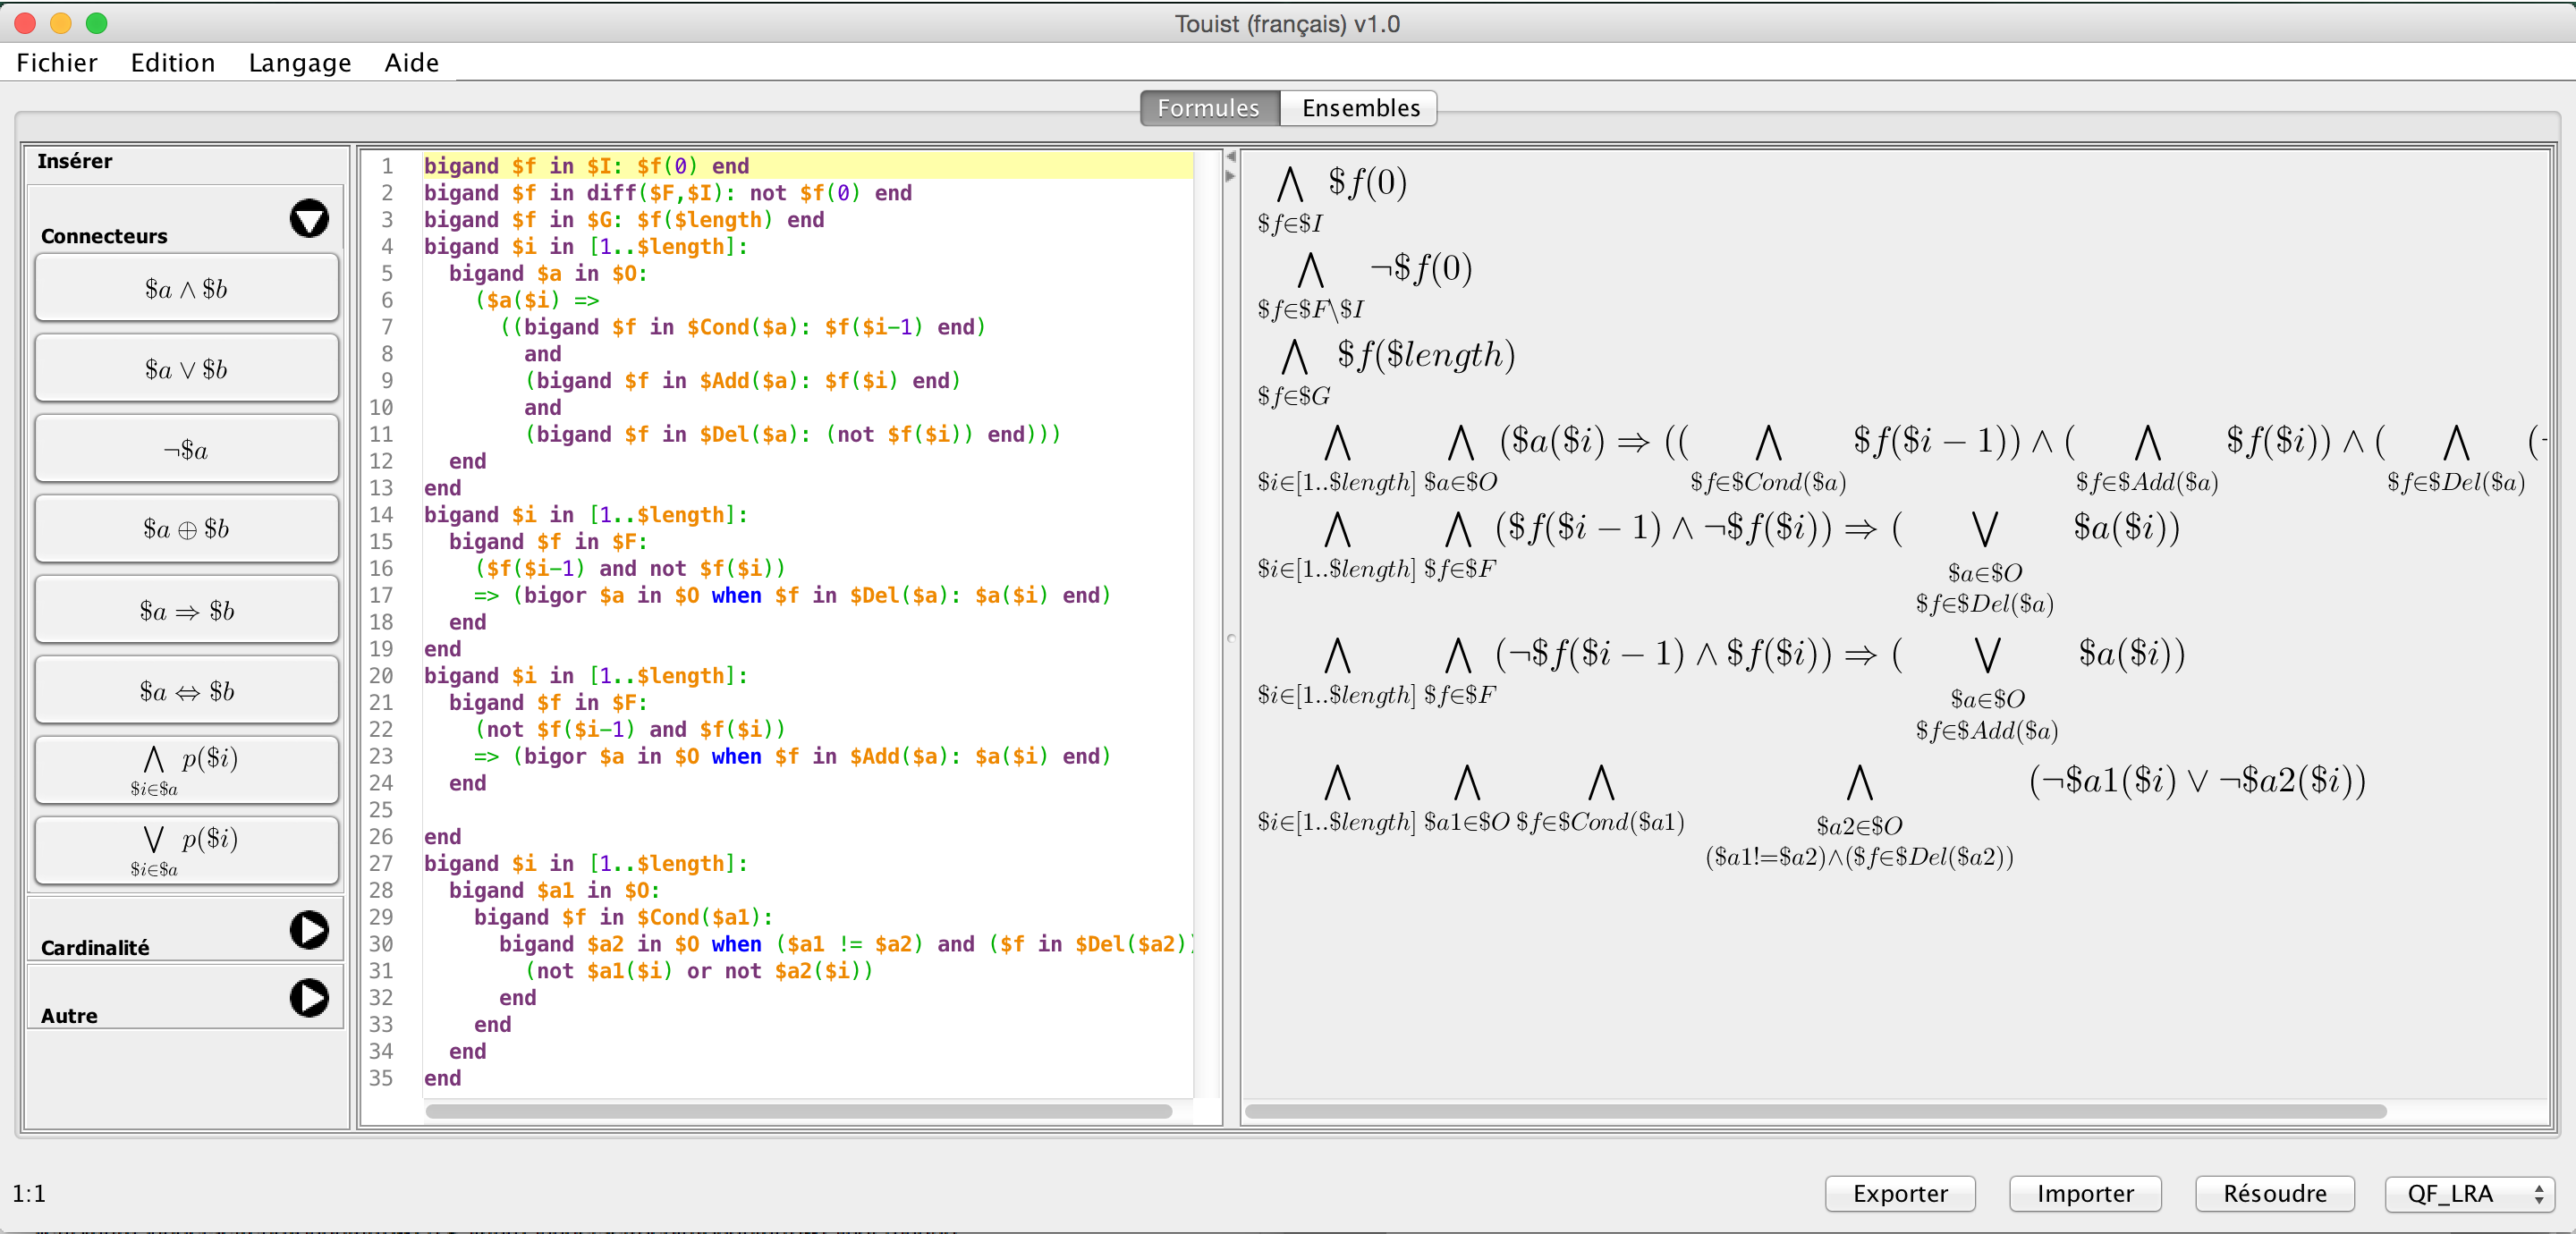
\includegraphics[scale = 0.3]{images/touist_planif.png}    
    \caption{Règles de codage (langage touistl à gauche et affichage \LaTeX\ à droite).}%
    \label{fig:touist-planif}% label for figure
  \end{figure}






La planification par satisfaction de base de clauses (planification SAT) a été introduite avec le planificateur SATPLAN \citep{kautzS92_planning_sat}. Dans cette approche, on travaille directement sur un ensemble fini de variables propositionnelles. Deux actions identiques pouvant apparaître à des endroits différents d'un même plan doivent pouvoir être différenciées et on leur associe donc des propositions différentes. Comme on ne connaît pas à l'avance la longueur d'un plan solution d'un problème, on ne peut pas créer un codage unique permettant de le résoudre puisqu'il faudrait créer une infinité de variables propositionnelles pour représenter toutes les actions de tous les plans possibles. La solution la plus commune consiste alors à créer un codage représentant tous les plans d'une longueur $k$ fixée. La base de clause ainsi obtenue est donnée en entrée à un solveur SAT qui retourne, lorsqu'il existe, un modèle de cette base. Le décodage de ce modèle permet alors d'obtenir un plan-solution. Si la résolution du codage ne donne pas de modèle, la valeur de $k$ est augmentée et le processus réitéré. Pour la complétude du procédé, tous ces modèles doivent correspondre exactement à tous les plans solutions d'une longueur fixée du problème.
Notre plate-forme de résolution de problèmes \nameTool est capable de prendre en compte à la fois des formules logiques et des \textit{ensembles de domaines}. Si notre objectif est de résoudre plusieurs problèmes de planification génériques, nous pouvons ainsi profiter de la flexibilité de \nameTool qui permet à l'utilisateur de décrire une méthode générique de résolution avec des règles encodées comme formules et d'utiliser des ensembles de domaines pour décrire chaque problème de planification particulier. De nombreuses règles de codage pour la résolution de problèmes de planification ont déjà été proposées \citep{kautzS92_planning_sat,MaliK99_plan_space_encodings,Rintanen:2006}. La figure~\ref{fig:touist-planif} présente l'intégration de l'un de ces codages dans \nameTool (codage dans les espaces d'états avec frame-axiomes explicatifs). La figure~\ref{fig:touist-sets} illustre les ensembles de domaines définis par \pddlmodule pour un problème particulier du célèbre monde des cubes "BlockWorld" et la figure~\ref{fig:touist-result} donne la solution renvoyée par le solveur.





   \begin{figure}[!ht]
    \centering 
     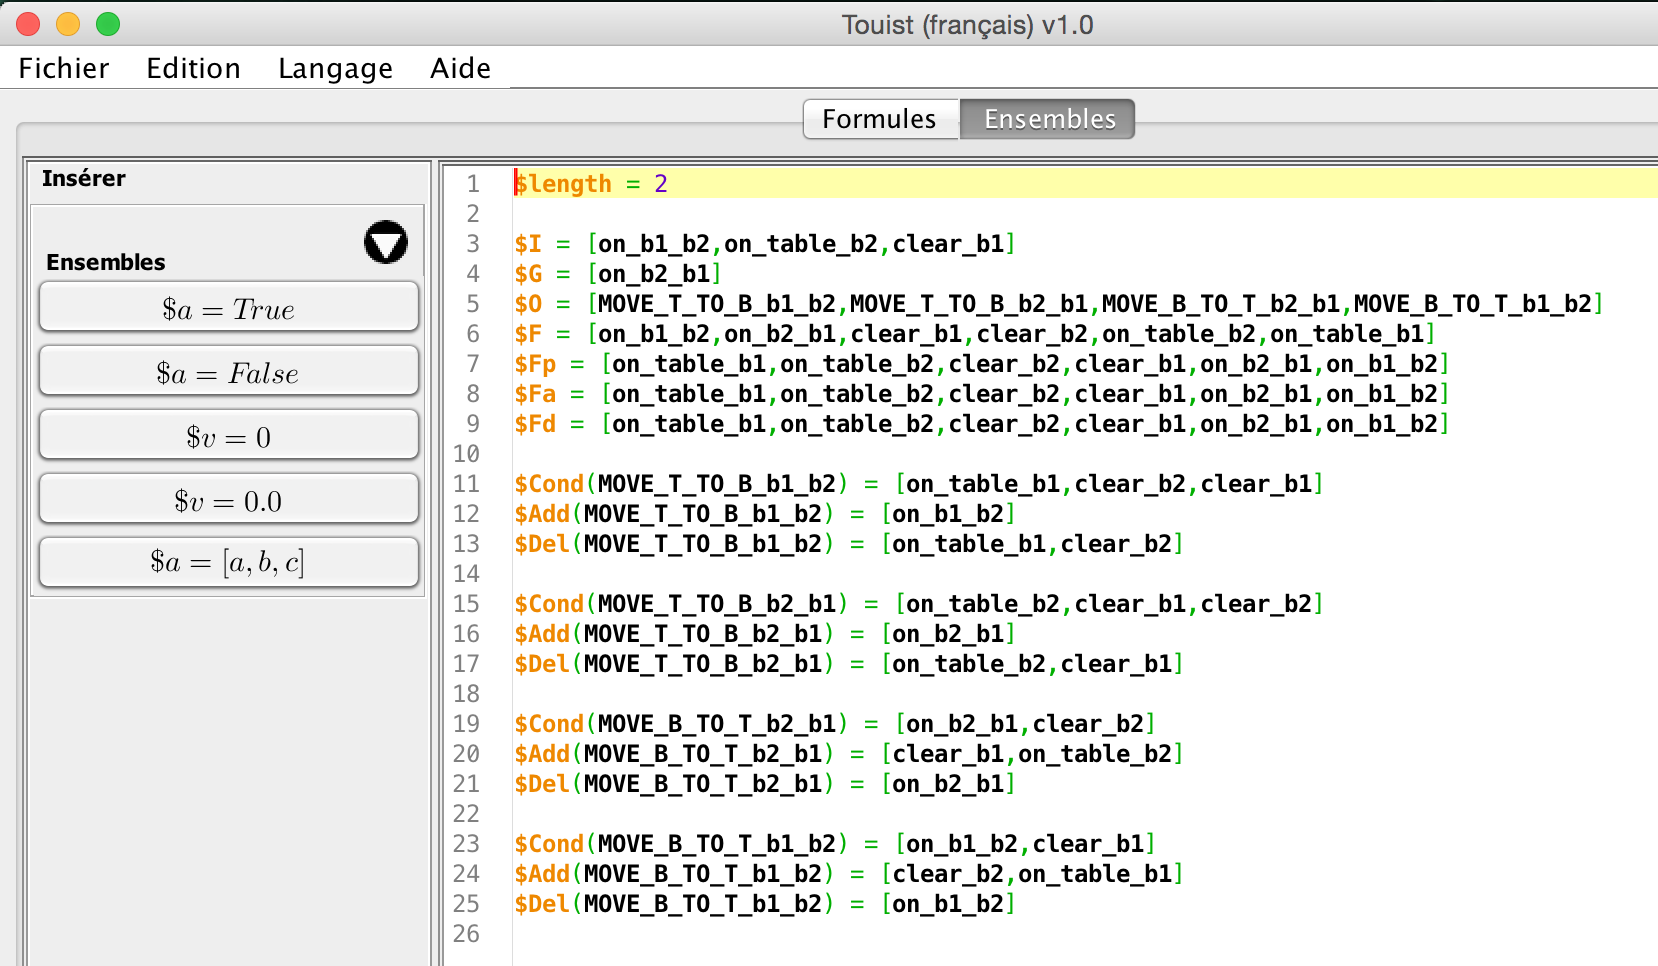
\includegraphics[scale = 0.3]{images/touist_sets.png}    
    \caption{Ensembles de domaines définis pour un problème de planification (BlocksWorld).}%
    \label{fig:touist-sets}% label for figure
  \end{figure}


   \begin{figure}[!ht]
    \centering 
     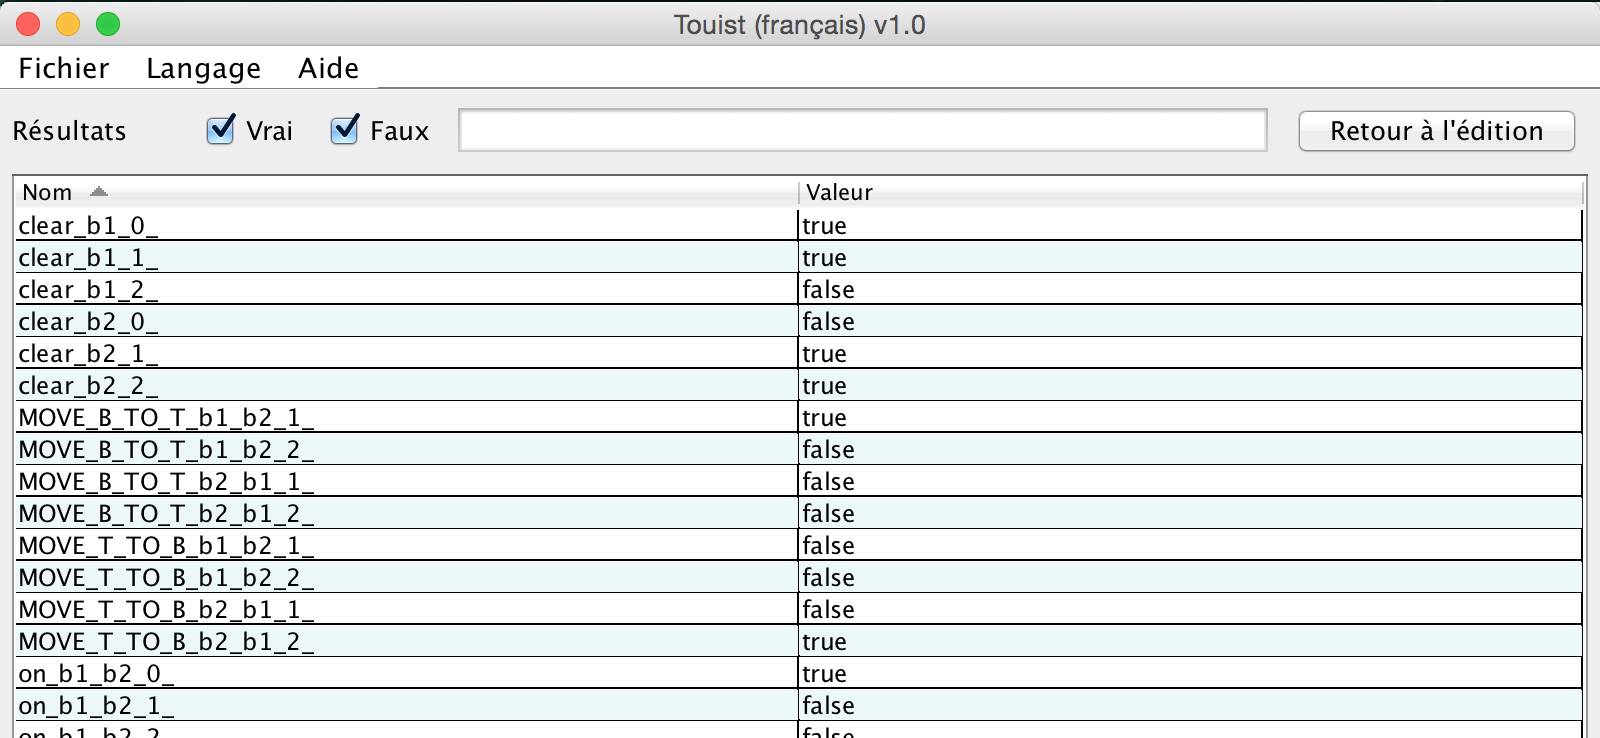
\includegraphics[scale = 0.3]{images/touist_result.png}    
    \caption{Solution renvoyée par le solveur (BlocksWorld).}%
    \label{fig:touist-result}% label for figure
  \end{figure}



Pour résoudre des problèmes de planification réels, l'une des principales difficultés à surmonter consiste à prendre en compte la dimension temporelle. En effet, de nombreux problèmes du monde réel nécessitent, pour être résolus ou exécutés plus efficacement, la prise en compte de la durée des actions, des instants auxquels des évènements se produisent, ou encore la concurrence d'actions.
En complément de SAT, notre plate-forme \nameTool est capable de gérer des théories comme la différence logique ou l'arithmétique linéaire sur les nombres entiers (QF\_IDL, QF\_LIA) ou les nombres réels (QF\_RDL, QF\_LRA), et d'appeler un solveur SMT pour trouver une solution. Pour être résolus, les problèmes de planification temporelle issus du monde réel nécessitent une représentation continue du temps, et donc, l'utilisation de nombres réels dans les codages logiques. \nameTool peut être utilisé pour résoudre de tels problèmes impliquant des actions avec durée, des évènements exogènes et des buts temporellement étendus, par exemple avec les règles de codage proposées dans \citep{MarisRegnier08}.









%
% Conclusion
%
%\section{Conclusion}



%
% Bibliographie
%





\bibliography{biblio}

\end{document}

